\section{Setup}
\begin{enumerate}
    \item Players decide amongst themselves which colour they wish to play.
    \item Each player takes six of the seven available cubes and mixes them up, rolling them onto the Grid.
    \item These cubes are then placed in the three middle columns of the bank behind the player's starting line in whichever configuration they see fit.
    \item Both players now roll the final cube and place it on The Grid in the middle of the row furthest away from their bank (see Figure~\ref{fig:setup}). This cube is known as the \textit{Grid Cube}.
\end{enumerate}
The player who rolled the highest number on their grid cube starts the game.

\begin{figure}[!h]
    \centering
    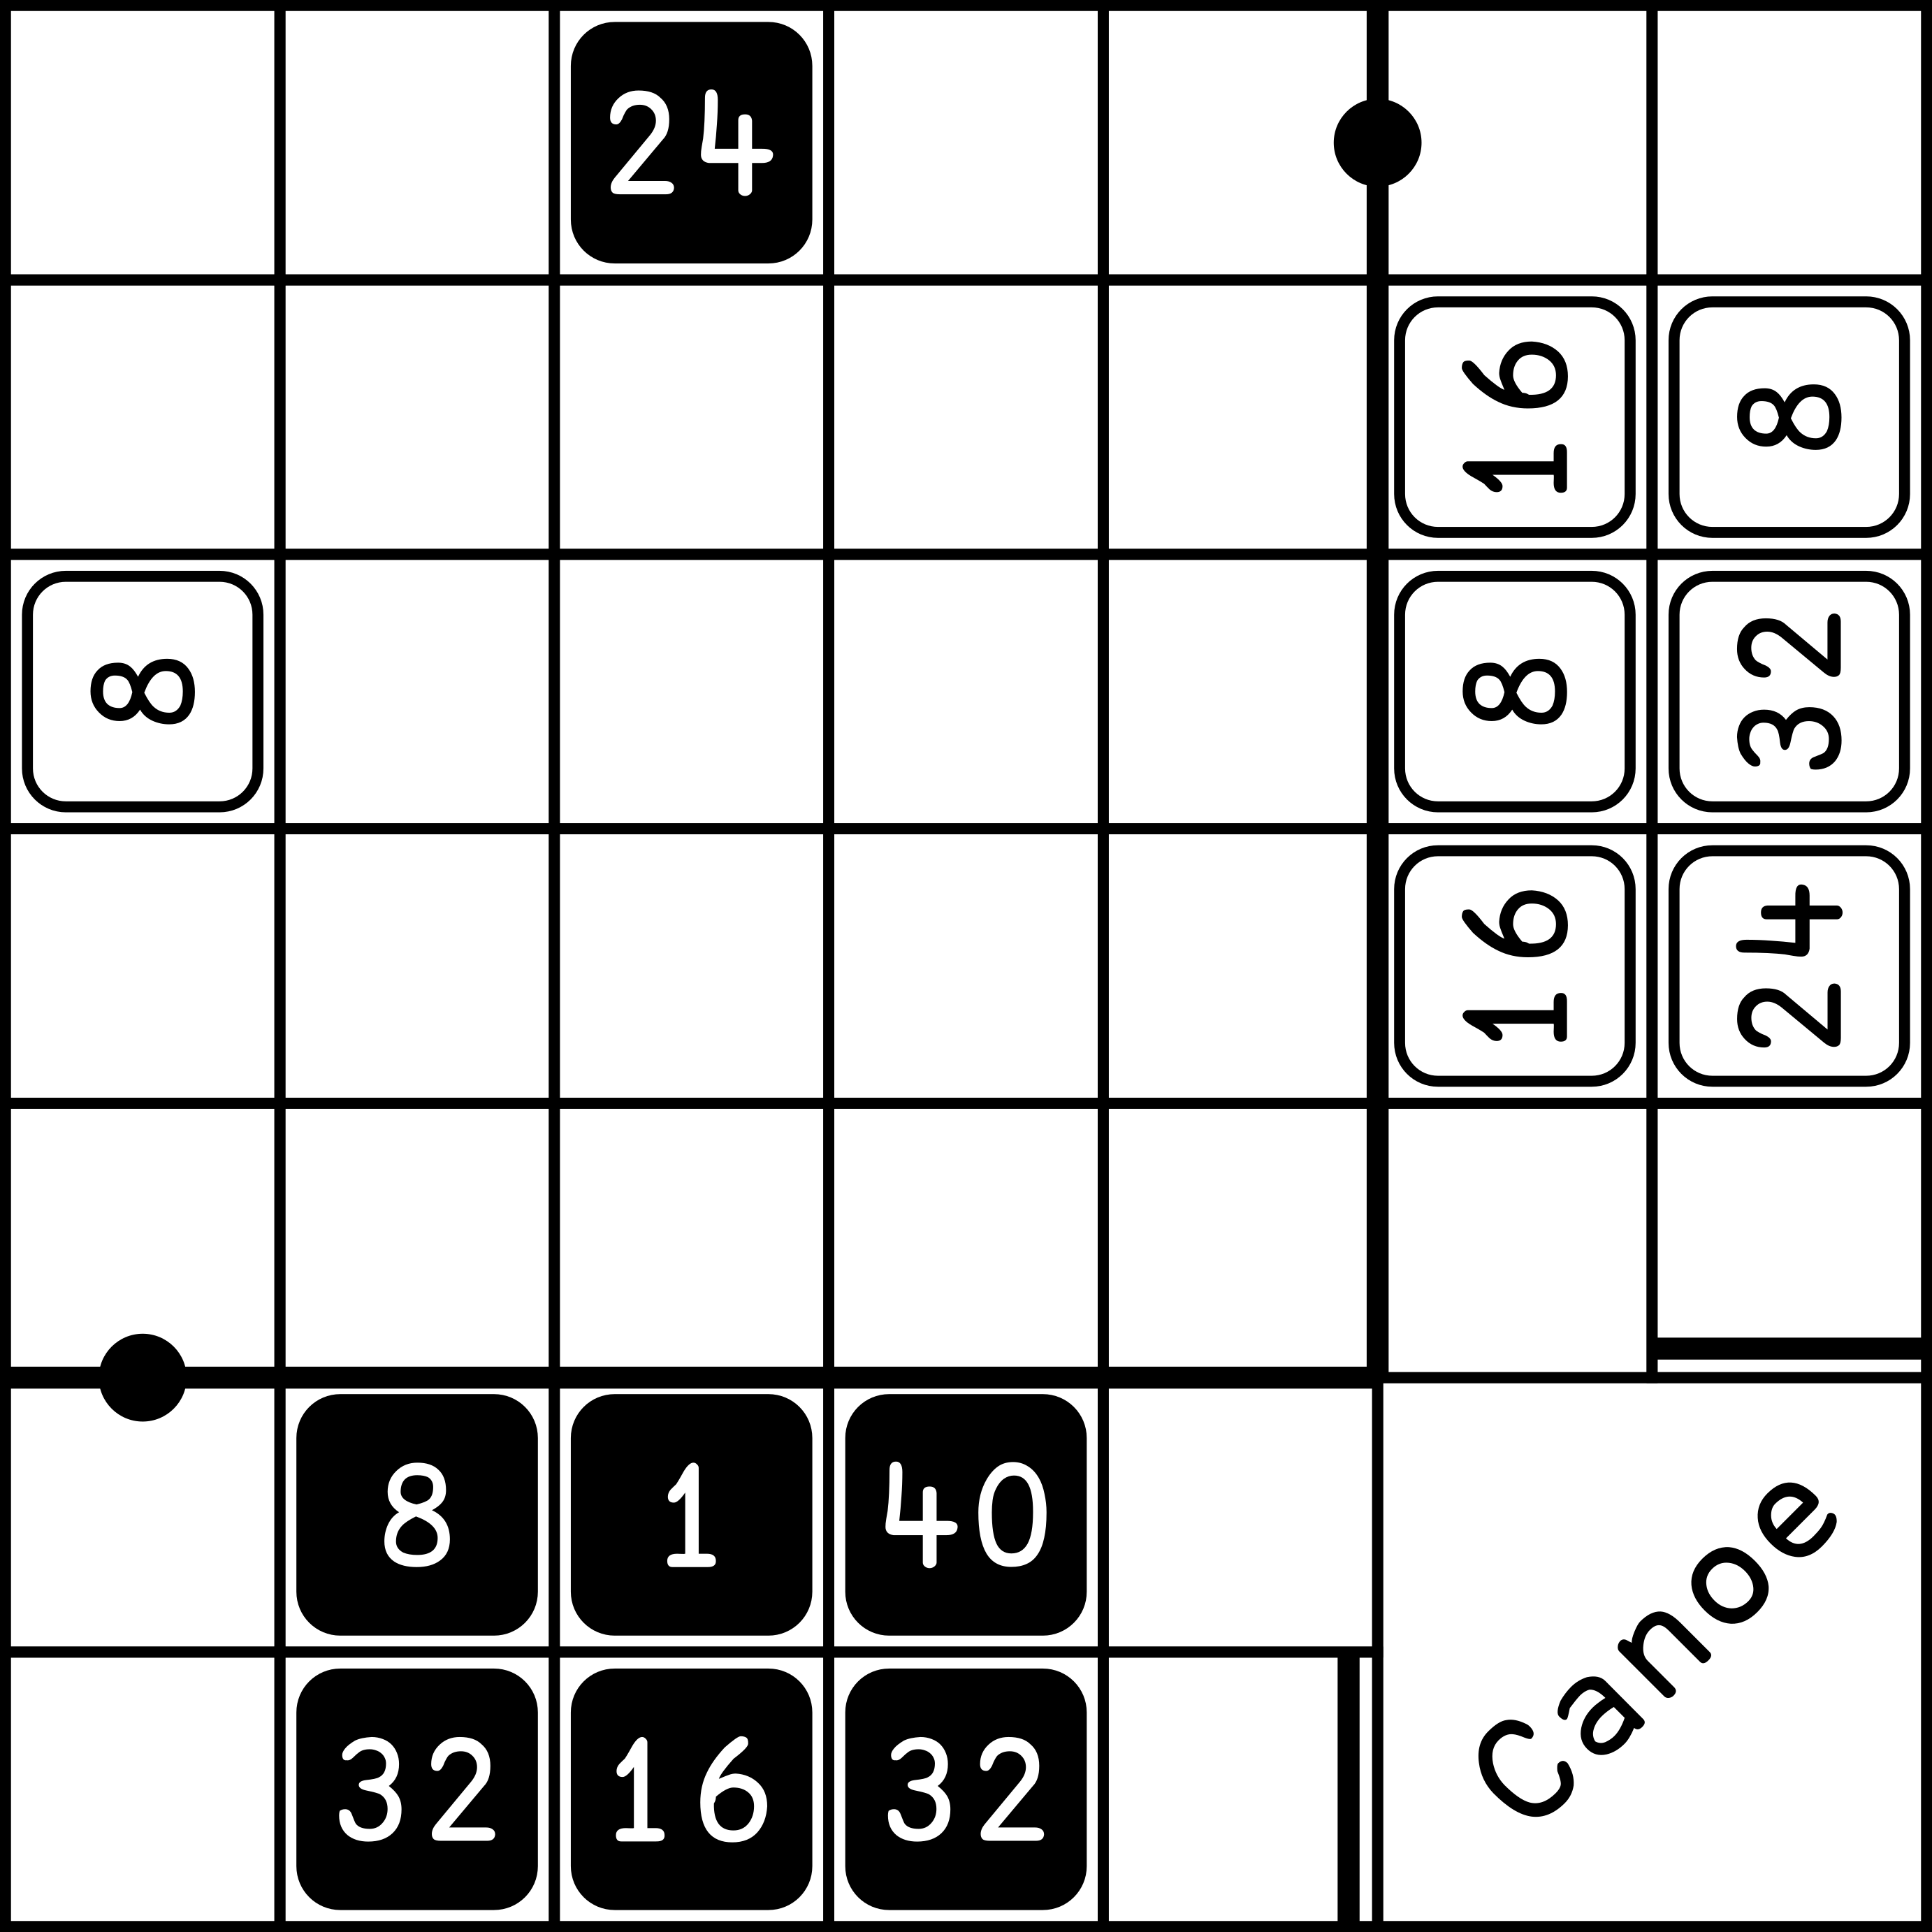
\includegraphics[width=8cm]{../graphics/setup}
    \caption{Example Setup}
    \label{fig:setup}
\end{figure}